\documentclass[12pt]{IEEEtran}
\usepackage{graphicx}
\usepackage{caption}
\usepackage{float}
\usepackage[style=ieee,backend=biber]{biblatex}
\usepackage[a4paper,margin=1in,footskip=0.25in]{geometry}
\usepackage[english]{babel}
\usepackage{pdfpages}

% uncomment for double spacing
\usepackage{setspace}
\onehalfspacing

\usepackage[autostyle]{csquotes}
\addbibresource{araspaper.bib}
\usepackage{hyperref}
\hypersetup{
    colorlinks,
    citecolor=black,
    filecolor=black,
    linkcolor=black,
    urlcolor=black
}

\begin{document}

\title{Connecting The Lab}
\author{
Jon Bakies, Mitchell Dunn, Elias Kapetanopoulos, and Magdy Ellabidy \\
Department of Computer Science and Networking \\
Wentworth Institute of Technology \\
Boston, MA 02115, USA \\
bakiesj@wit.edu, dunnm8@wit.edu, kapetanopoulose@wit.edu, ellabidym@wit.edu
} 

\maketitle
\clearpage


\section{Network Design}
The network design consists of two firewall routers, a switch, Raspberry Pi, and two ESXi clusters.
Each router has a connection to the internet with their own IP address and a shared IP address for redundancy with CARP.
The routers have the same setup for the internet network as well.
It is good practice to have a dedicated line between the routers so they can synchronize routing tables and other data for a seamless transition should one of the routers fail.
Unfortunately, both of the routers have a broken NIC, so we have to rely on synchronizing over LAN.
Although this isn't best practice, it is still a reliable way to set up redundancy.



\begin{figure*}[t]
	\centering
	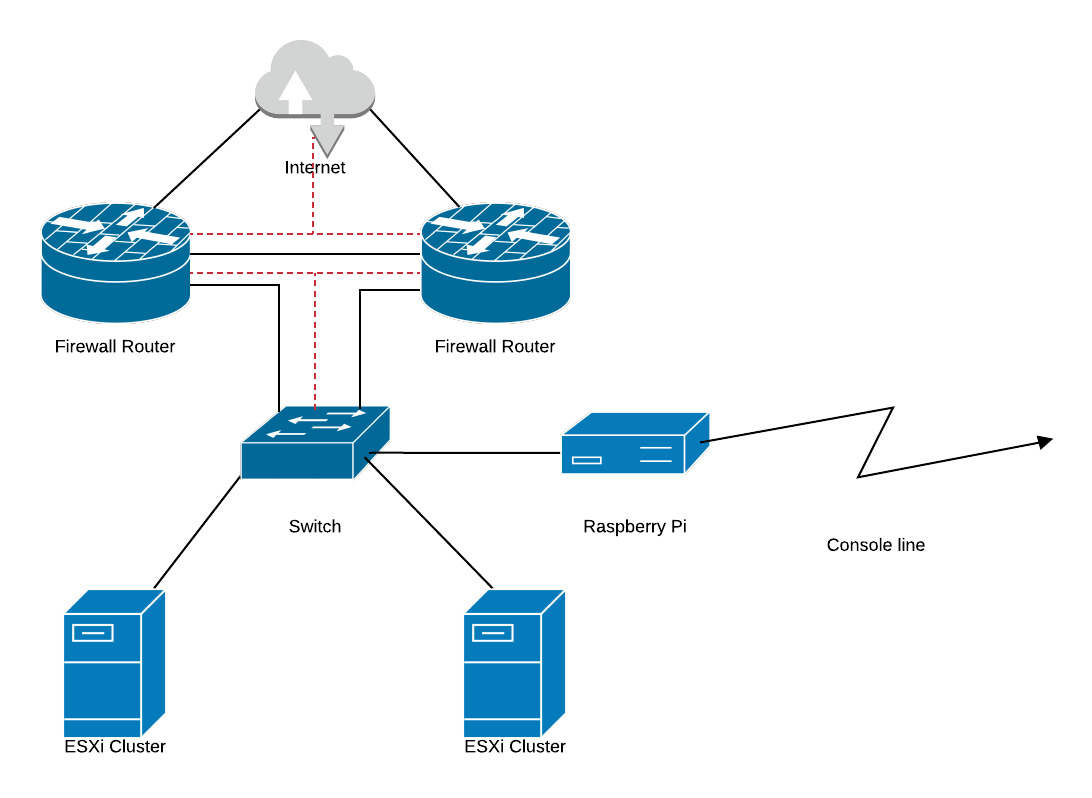
\includegraphics[width=\textwidth]{topology.png}
	\caption{Network Topology}
\end{figure*}

\section{Serial Over LAN}
\subsection{ser2net}
Ser2net is a daemon that opens a TCP or Telnet connection to the server's serial ports.
After connecting all of the devices' communication ports to the Raspberry Pi ser2net allows for a single telnet connection to each device.
There are some nuances that come along with this daemon.
Ser2net does not provide a service for SSH, so the communication between the user and the device will be unencrypted.
Although SSH would be preferred, a telnet connection is acceptable because in order to access the Serial over LAN (SoL) a user has to VPN into the network.
The only way to access the network is physically or via a secure connection.
Another nuance is the configuration.
The way ser2net opens a connection to the serial ports is by the device in the /dev directory.
The devices in the /dev directory are named by the order in which they are plugged in, meaning the needs to be an order in which they are plugged in.
\subsubsection{Configuration}
The default ser2net config file is located at /etc/ser2net.conf.
The configuration file defines all of the connections ser2net provides.
An example of connection for this SoL project is \textit{192.168.1.12,5560:telnet:0:/dev/ttyUSB1:9600 8DATABITS NONE P5R3 remctl}.
It is broken into parts \textit{\textless network port\textgreater :\textless state\textgreater :\textless timeout \textgreater :\textless device\textgreater :\textless options \textgreater} 
\cite{ser}.
The network port defines the end point a user will use to connect to the serial port.
The state option is used to determine the protocol used to communicate with the serial port.
The third option is the timeout in seconds.
The will be disconnected if there are this many seconds of no activity.  
This option is used to prevent inactive users from blocking others from using the device.
After timeout is the device, which as previously discussed is located in the /dev directory.
The final part is designated for options, separated by space.
Options for this project are specifically for a Cisco console device.
The P5R3 option is the name of a banner created earlier in the file that lets the user know which device they're connected to. 

\subsubsection{Installation}
ser2net is available on the apt package manger, so install is simple.

\textit{apt install ser2net}
\subsection{USB hub}
The USB hub is used to limit the wires run to the server room.
All of the devices in the pod are connected to the USB hub.
Because there are currently at most 9 devices in a pod, a 13 port hub is used.
In order to constantly have the same device number, the devices need to be plugged in a specific configuration.
Figure 2 shows a mockup of the usb hub.
Each used port is labeled with the device that is plugged into it and the phsycial port address used by the hub.
These are important to note because they are what determine ser2net's configuration.
The port number describes the physical port of the device atached, which is directly mapped to the device file.
The relationship between device and port is very important and should be standardized.

\subsection{USB-RJ45 Converter}
The USB hub is plugged into a USB to RJ45 converted to extend the connection into the server room.
The reason this is needed is because a USB cable is rated for only 5 meters in length without a repeater.
RJ45 on the other hand has a much longer rating of 100 meters, which is more than sufficient for the lab set up.
After the RJ45 line is run into the server room, it will be converted back into USB and plugged into a port on the Raspberry Pi.

\subsection{Naming Scheme}
The device names are determined by pod number, device type, and device number.
Pods are numbered 1 through 5.
For perspective, we are standing at the front of the room looking at the server room.
Pod 1 will be the left most pod that is closest to the front of the room.
The pod number will continue to increment in a left-to-right, front-to-back fashion.
Once the pod number is designated, the devices are named in a similar way.
Starting at the top most device in the front facing door (away from the server room) of the pod, devices names are incremented going to the bottom device and wrapping to the top of the back side.
The devices are designated with an S if it is a switch, and an R if it is a router.
The final device name should look like like P1S1.

\subsection{Raspberry Pi}
The Raspberry Pi acts as the SoL server.
It is running the ser2net daemon and hosts all the connection to the serial devices.
For ease of use for the user, the Raspberry Pi has a virtual interface for each device with its own IP address.
Each of these addresses is given a hostname by the DNS server on the router.
This allows the user to telnet to the device by the given device name described in the Naming Scheme section rather than the IP address.
On the Pi is a bash script to make setup simple for the sysadmin.
This script creates a ser2net configuration file, creates all the virtual interfaces, and makes a file containing all the IP address mapped to the correct device name.
More documentation of the script will be supplied in the the actual an on the git repo.

\begin{figure*}[t]
	\centering
	\makebox[\textwidth]{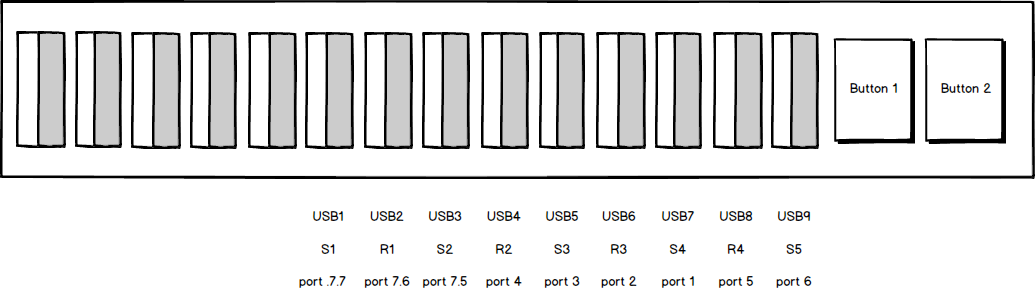
\includegraphics[width=\textwidth]{usbports.png}}
	\caption{USB hub mockup}

\end{figure*}

\section{Routers}

\subsection{Overview}
The routers and firewalls for this environment are configured with the OPNsense firewall software \cite{opnsense}.
The software is highly configurable and provides state of the art security and software that adds convenience and usability to the network.
Many of the software packages available in OPNsense are utilized in the network in order to achieve the goals set out for this project.
OPNsense is developed to be an easy-to-use firewall based on the FreeBSD project, it was designed to be able compete with the features present in commercial firewalls but using open source software.
The OPNsense software is a fork of pfSense \cite{pfsense} that has a focus on timely security updates as well as code quality and security \cite{opnsenseabout}. 

\subsection{Services}
\subsubsection{DHCP Server}
The DHCP server is meant to provide convenience to network users and admins.
It will hand out addresses to new hardware added to the network for the ease of configuration. 
Since a lot of software has some kind of web configuration the DHCP server allows us to connect to the web configuration to provide a static address if desired. 
The pool of addresses handed out by the DHCP server is high numbered while the static addressed that are assigned to servers and software are low numbers. 
The DHCP server also provides convenience when connecting to the network physically, there is no need to assign a computer connecting a static IP address. 

\subsubsection{OpenVPN Server}
The OpenVPN server is meant to allows students, admins, and professors to connect to the environment from anywhere on the internet. 
It is setup as a remote access and uses a pre-shared key as well as a username and password combination for authentication.
The usernames and passwords are configured through the OPNsense local database and can be managed through the OPNsense web configuration.
OPNsense provides some useful features to manage accounts that will be helpful in this environment.
As an example, the accounts can be set to expire which is useful when setting up a student account that will only have access for one semester. 
OPNsense will automatically make the keys needed for a user to connect to the VPN server during account creation. 
OPNsense also provides a wizard to export the OpenVPN configuration files necessary for a user to connect to the server. 
Since the users are connecting with a username and password, logs can be audited to find out when a user was connecting if necessary. 

\subsubsection{DNS Resolver}
The DNS Resolver is another service that provides convenience for the users on this network. 
We are utilizing the DNS resolver to simplify connecting to the hardware in the network as described in the Serial Over LAN section of this paper. 
When connecting to the VPN the DNS server is specified upon connecting and this tells the clients to send any DNS traffic to our resolver. 
Since the DNS traffic is coming to our firewall we are able to resolve hostnames for a local domain.
We use this to provide a unique hostname for each IP address used in the ser2net configuration. 
This means a user can use a descriptive name to connect to a specific router or switch in a specific pod very easily.
Names are also provided for the hosts in the ESXi cluster, the remote management for the Dell hardware, the OPNsense firewalls themselves, and any hostnames specified in DHCP requests.

\subsection{Redundancy}
\subsubsection{CARP}
The Common Address Redundancy protocol is utilized to provide an address that is shard between the two firewalls in the network.
The firewalls have a shared address on both the WAN, 69.43.72.202, and the LAN, 10.123.18.1, as well as their own unique IP address on each network.
Maverick's WAN interface has an IP address of 69.43.72.203, and it's LAN interface is 10.123.18.2.
While Goose's WAN interface has 69.43.72.204, and it's LAN interface has 10.123.18.3. 
The unique addresses are necessary in order to direct traffic needed to go to a specific host, such as pfSync or XMLRPC traffic, can still be routed correctly. 
In the event of one of the firewalls becoming inoperable the other firewall will immediately take the responsibility of routing any traffic for the shared addresses.
\subsubsection{pfSync}
The pfSync protocol is responsible for synchronizing the connection states of any TCP or UDP connections being made through the firewall.
This is to make sure connections can be resumed without interruption in the case of a firewall going down. 
Without pfSync running the connections would have to be reset if the primary firewall went down. 
\subsubsection{XMLRPC Sync}
The responsibility of the XMLRPC synchronization is to sync the configuration of all the services from the primary firewall to the secondary as well as any state those servers are in.
The primary firewall will continually update the secondary firewall with any changes in configuration to any services as well as any state that the running services are in.
If the primary firewall were to go down the secondary firewall is able to immediately replicate any of those services. 
This service syncs all of the services we are utilizing in the firewall. 
\begin{itemize}
\item Local Database Users and Groups
\item Certificates, used by the VPN and web configuration
\item Firewall and NAT rules
\item DHCP configuration and states
\item Any defined routes in the routing table
\item CARP configuration and virtual IP addresses
\item Custom DNS entries
\item OpenVPN configuration
\end{itemize}

\subsubsection{NAT}
The firewalls in this environment provide a NAT service like most routers to provide hosts on the LAN to have connections with any address on the internet. 
The NAT rules were written manually in order to use the shared address in the CARP setup to provide a redundant path to the internet for the hosts on the LAN.
Since the states of all connections happening through the NAT are duplicated on the other router using pfSync, described earlier, the connections with the internet are not interrupted in the case of a firewall going down. 
The NAT configuration on the firewalls can also provide port-forwarding if any services running on the LAN were desired to be accessible over the internet.  

\section{ESXi Hosts}
There are two ESXi Hosts in the environment that will be used to provide virtual machines for use by anyone that could find them useful. 
There was discussion of hosting networks of virtual machines for students to practice routing and switching or securing the network for a security class. 
Currently the networking is setup for only connecting to the existing subnet (10.123.18.0/24) and VMs that are connected to the ESXi's virtual switch will be given DHCP leases by default. 
In the future VLANs can be utilized to provide more isolated virtual machine hosting and prevent any kind of issues that a student may cause configuring some networking within the environment.

\newpage \section{References} \printbibliography[heading=none]
\textit{USB Hub purchase link: https://www.amazon.com/gp/product/B00HL7Z46K/ref=oh_aui_detailpage_o01_s00?ie=UTF8&psc=1}

\textit{USB-RJ45 converter purchase link: https://www.amazon.com/gp/product/B003L14ZTC/ref=oh_aui_detailpage_o01_s00?ie=UTF8&psc=1}


\textit{git repo: https://github.com/mitchjdunn/ser2netHelper}
\end{document}
